\documentclass[crop,tikz]{standalone}
\usepackage{float}
\usepackage{tikz}
\usetikzlibrary{arrows.meta}
\usepackage{amsmath}
\usepackage{xcolor}
\usepackage{bm}
\let\oldbm\bm
\renewcommand{\bm}[1]{\oldbm{#1}}
\definecolor{gray}{RGB}{200,200,200}

\begin{document}    
    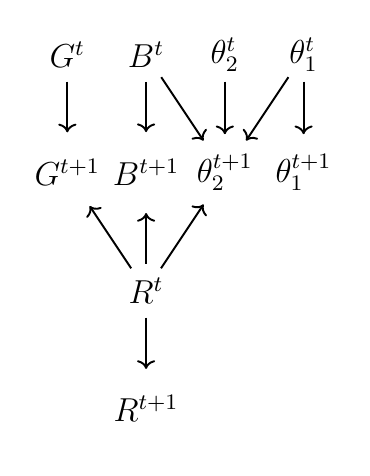
\begin{tikzpicture}
        \node[circle, inner sep=0.12em] (rt) at (1,-1.5) {\large$R^t$};
        \node[circle, inner sep=0.12em] (gt) at (0,1.5) {\large$G^t$};
        \node[circle, inner sep=0.12em] (bt) at (1,1.5) {\large$B^t$};
        \node[circle, inner sep=0.12em] (2t) at (2,1.5) {\large$\theta_2^t$};
        \node[circle, inner sep=0.12em] (1t) at (3,1.5) {\large$\theta_1^t$};
        

        \node[circle, inner sep=0.12em] (rtt) at (1,-3) {\large$R^{t+1}$};
        \node[circle, inner sep=0.12em] (gtt) at (0,0) {\large$G^{t+1}$};
        \node[circle, inner sep=0.12em] (btt) at (1,0) {\large$B^{t+1}$};
        \node[circle, inner sep=0.12em] (2tt) at (2,0) {\large$\theta_2^{t+1}$};
        \node[circle, inner sep=0.12em] (1tt) at (3,0) {\large$\theta_1^{t+1}$};
        
                
        \begin{scope}[]
            \draw[->, line width = 0.7] (rt) edge[] (rtt);            
            \draw[->, line width = 0.7] (gt) edge[] (gtt);
            \draw[->, line width = 0.7] (bt) edge[] (btt);
            \draw[->, line width = 0.7] (1t) edge[] (1tt);
            \draw[->, line width = 0.7] (2t) edge[] (2tt);

            \draw[->, line width = 0.7] (rt) edge[] (btt);
            \draw[->, line width = 0.7] (rt) edge[] (gtt);
            \draw[->, line width = 0.7] (rt) edge[] (2tt);

            \draw[->, line width = 0.7] (1t) edge[] (2tt);
            \draw[->, line width = 0.7] (bt) edge[] (2tt);
        \end{scope}
    \end{tikzpicture}


\end{document}